\documentclass[10pt,a5paper]{article}
\usepackage{graphicx}
\usepackage{hyperref}
\usepackage[utf8x]{inputenc}
\usepackage{polski}

\usepackage{geometry} 
\newgeometry{tmargin=1cm, bmargin=1.5cm, lmargin=1cm, rmargin=1cm}



\begin{document}

\begin{titlepage}
\begin{center}

\huge
{\tt Ninetails (9tails)}

\Large
Skrócona instrukcja obsługi

\vspace*{2cm}

\normalsize
Niskobudżetowy akcelerator dla komputera Amiga 600.

\vspace*{2cm}
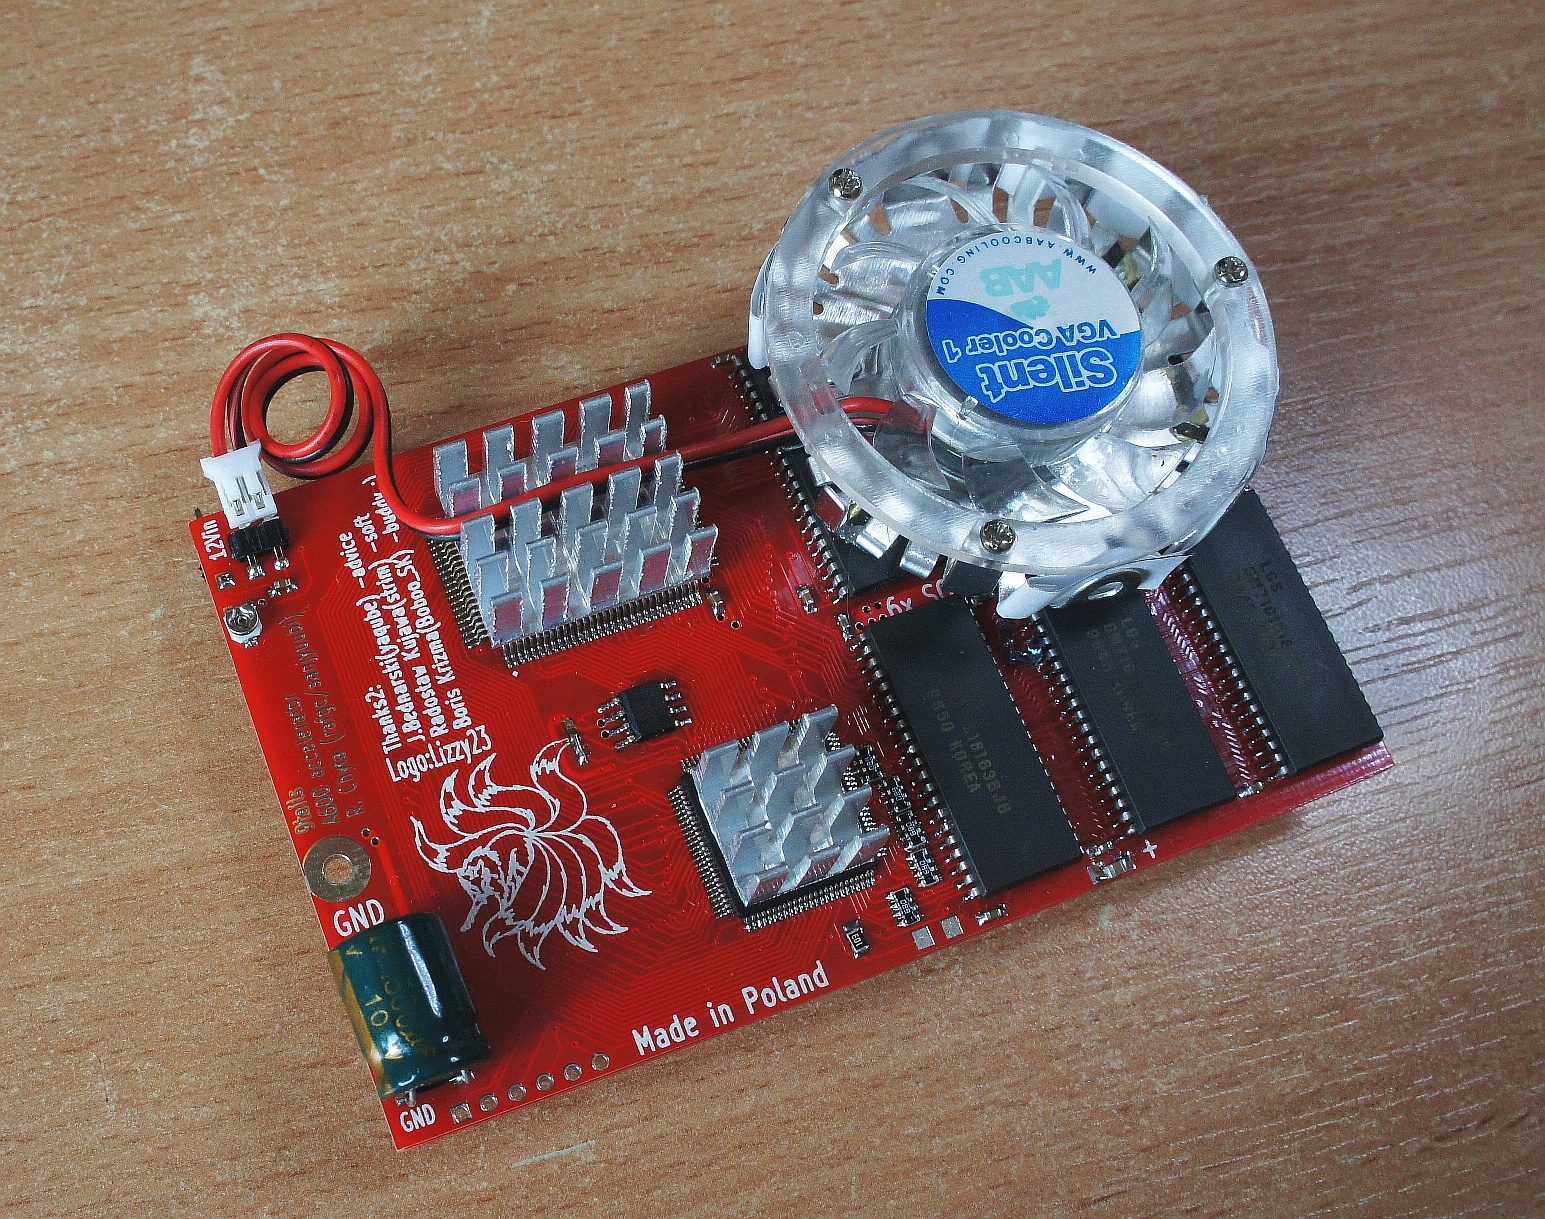
\includegraphics[scale=0.15]{ninetails-photo.jpg}
\vfill

\normalsize
\today

\end{center}
\end{titlepage}

\section*{Wprowadzenie}

Dziękujemy za wybranie naszego akceleratora, który charakteryzuje się następującą specyfikacją:

\begin{itemize}
	\item Procesor Motorola MC68EC020FG25 taktowany 28MHz
	\item Łączna ilość pamięci wynosi 11MB - 8MB FAST(autoconfig), 1.5MB SLOW oraz 1.5MB pamięci dodawanej do systemu przez narzędzie konfiguracyjne 9tcfg.
	\item Funkcje mapowania kickstartu z pliku (maprom) oraz krycia kickstartu (shadowrom - rom shadowing).
	\item Możliwość wyłączenia 4MB z obszaru \$600000-\$9FFFFFF celem uzyskania bezkonfiktowego dostępu do PCMCIA.
	\item Możliwość wyłączenia karty z poiomu oprogramowania, nie trzeba instalować przełącznika.
\end{itemize}

\begin{center}
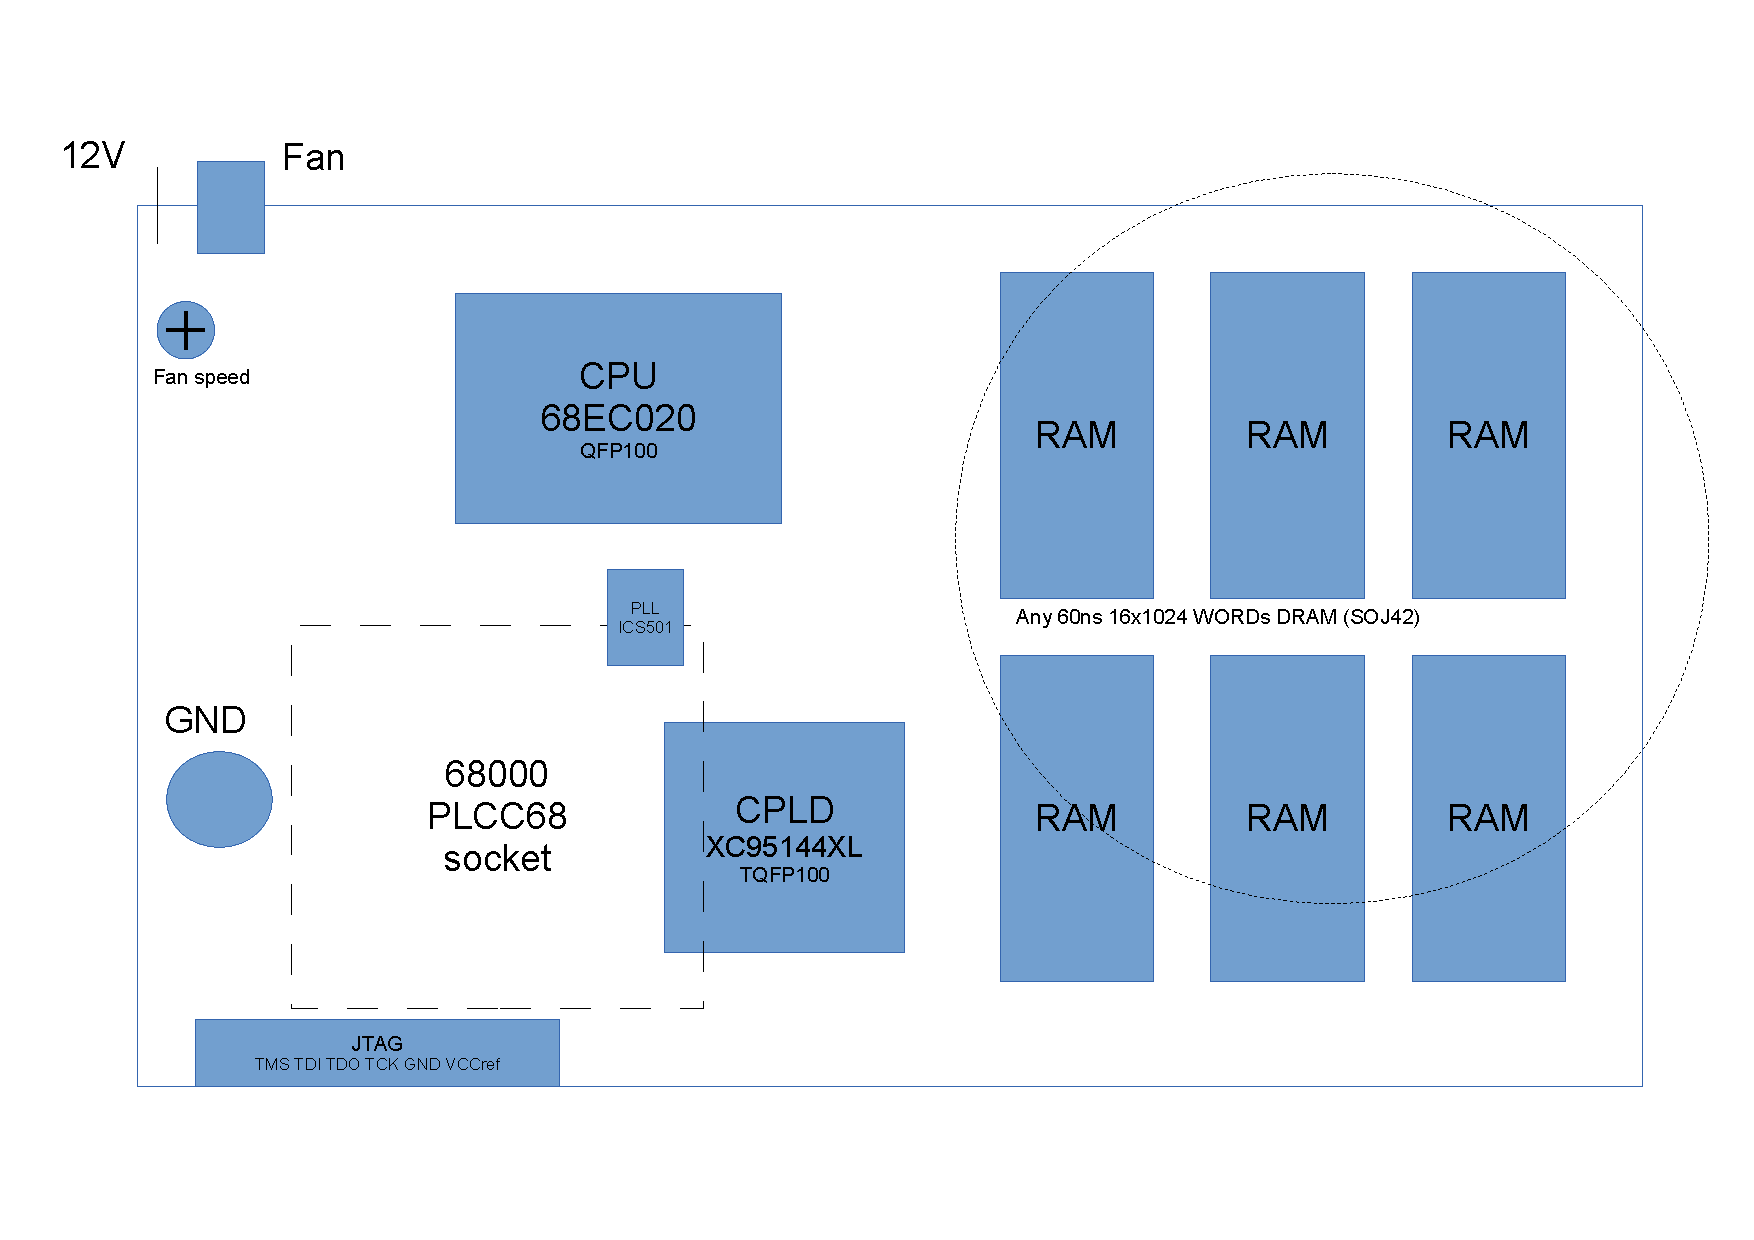
\includegraphics[scale=0.25]{ninetails-drawing.pdf}
\end{center}

Z powodu ograniczeń przestrzennych, nie jest możliwe zamontowanie sanek na dysk twardy, co wymusza na użytkowniku konieczność
umocowania go w innym miejscu lub zastąpienia kartą CF. 

Z powodu wydzielania przez procesor dużej ilości ciepła, proszę o rozwagę przy próbach modyfikacji chłodzenia.

\section*{Montaż}

Instalacja karty jest banalna, jednak proszę o zachowanie ostrożności. W skład zestawu wchodzą:

\begin{itemize}
	\item Akcelerator.
	\item Przewód z sondą podpinaną do napięcia 12V w gnieździe zasilającym.
	\item Śrubka (wkręt) i  plastikowa tuleja.
	\item Dyskietka rozruchowa z programem 9tcfg (opcjonalnie).
	\item Instrukcja (opcjonalnie).
\end{itemize}

\noindent W celu zamontowania karty, należy wykonać poniższe kroki:

\begin{itemize}
	\item Otworzyć komputer.
	\item Nałożyć kartę na procesor MC68000FN8. Złącze 12Vin powinno być skierowane w stronę tylnej ściany komputera. Zalecane jest uprzednie spryskanie nóżek procesora czystym spirytusem lub izopropanolem i założenie karty "na mokro". Proszę nie używać spirytusu salicylowego.
	\item Podłącz zasilanie wentylatora 12V poprzez zapięcie sondy na szynie złącza zasilacza oraz nasuwając konektor na wystający PIN 12Vin w karcie.\\
	\begin{center}
	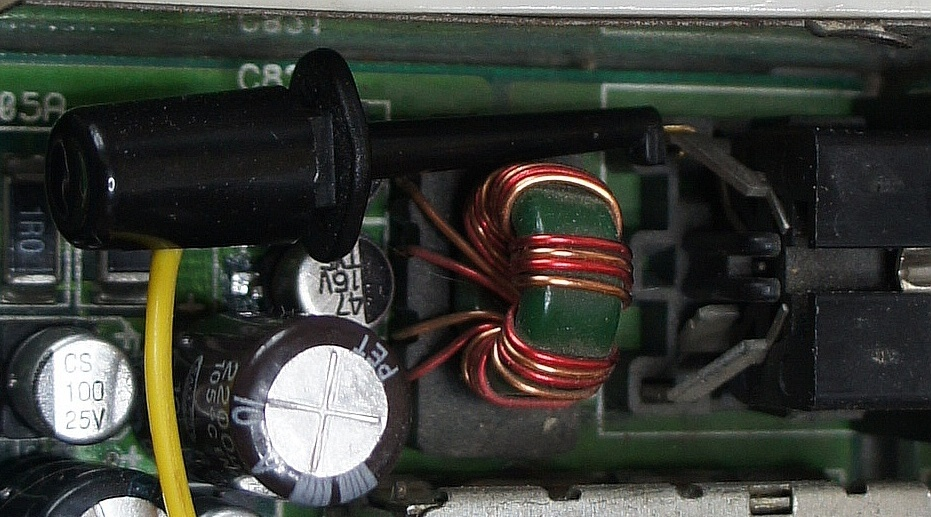
\includegraphics[scale=1]{probe.jpg}
	\end{center}

	\item W miejscu gdzie znajduje się otwór montażowy sanek, włóż tuleję z tworzywa sztucznego pod kartę  i wkręć śrubę od góry. W niektórych przypadkach może być wymagane podszlifowanie tulei jeśli jest za wysoka, lub podłożenia podkładki z papieru, gdy jest za niska. Śruba nie musi być mocno skręcona.
	\item Złóż komputer.
\end{itemize}


Amiga powinna się uruchomić bez żadnych dodatkowych czynności, jeśli uruchamiasz komputer z dysku twardego, na belce workbencha, w zależności od ilości zainstalowanych dodatków powinno automatycznie ukazać się około 8-9MB wykrytej pamięci. Typ procesora można sprawdzić poleceniem {\tt cpu}, zaś ilość dodanej pamięci do systemu poprzez polecenie {\tt avail}.

Aby w pełni wykorzystać możliwości karty, należy skorzystać z narzędzia  {\tt 9tcfg}. Można je pobrać z \url{http://rkujawa.github.io/9tweb/}. Kod źródłowy programu jest dostępny z poziomu repozytorium GitHub \url{http://github.com/rkujawa/9tcfg/}.

\section *{9tcfg - podstawowa obsługa}

Jak już wspomniano wcześniej, do aktywowania niektórych funkcji jakie oferuje karta, wymagane jest użycie narzędzia 9tcfg. Narzędzie to umożliwia wyłączenie karty programowo, włączeniu trybu kompatybilności z PCMCIA okupionego zmniejszoną ilością wykrywanej pamięci o 4MB, dodawanie do systemu dodatkowej pamięci o rozmiarze 1.5MB (1+ 0.5),  czy też najważniejszej opcji dla ludzi pracujących w systemie, czyli maprom lub shadowrom. Pełną listę poleceń otrzymamy wpisując {\tt 9tcfg help}. Oto kilka przykładów:

\begin{itemize}
\item {\tt 9tcfg m68k on} - wyłącza kartę, po resecie amiga uruchomi się z zdezaktywowanym akceleratorem
\item {\tt 9tcfg pcmcia on} - amiga po resecie uruchomi się z ilością pamięci pomniejszoną o 4MB na rzecz kompatybilności z PCMCIA
\item {\tt 9tcfg moremem} - dodaje do systemu dodatkowe 1.5MB
\item {\tt 9tcfg instcache off} - wyłącza cache instrukcji procesora sprzętowo, czasami pomocne przy uruchamianiu dem z dyskietek jak "State of Art"
\end{itemize}

Polecenia można ze sobą łączyć. Począwszy od wersji 1.2, można umieszczać 9tcfg w pliku startup-sequence np. do zautomatyzowania procesu mapowania kickstartu i dodawania dodatkowej pamięci, tak jak w poniższym przykładzie:



{$$\tt 9tcfg \  maprom \  on \  loadrom=KSX.X.rom \  moremem \  reboot \  \rangle NIL:$$}


\section*{Podziękowania}

Akcelerator Ninetails (9tails) został zaprojektowan przez Rafała Chyła (rafgc/sanjyuubi). Narzędzie konfiguracyjne zostało napisane przez  Radosława Kujawę  (strim).\\

Podziękowania należą się: Jakubowi  Bednarskiemu (yaqube), Borisowi  Krizma (Boboo\_SK), Radosławowi Kujawie (strim) oraz użytkownikowi deviantart.com Lizzy23 za zgodę na użycie swojej pracy jako loga na płytce PCB.


\section*{Warunki korzystania}
Pomimo próby uzyskania jak największej kompatybilności, nie ma możliwości zagwarantowania w 100\% bezbłędnej pracy. W związku z powyższym, używasz produktu na własne ryzyko. Autor akceleratora, jak również autor oprogramowania nie biorą odpowiedzialności, za ewentualne szkody.

\end{document}
